\documentclass[11pt,a4paper]{article}

\usepackage[margin=22mm,headheight=14pt]{geometry}

\usepackage{longtable,booktabs,array,hyperref,xcolor,tikz,fancyhdr}

\usepackage{fontspec,xeCJK}

\setmainfont[Ligatures=TeXOff]{Times New Roman}

\setsansfont[Ligatures=TeXOff]{Times New Roman}

\setmonofont[Ligatures=TeXOff,WordSpace={1,1,1}]{Times New Roman}

\setCJKmainfont{Noto Serif CJK SC}

\setCJKsansfont{Noto Serif CJK SC}

\setCJKmonofont{Noto Serif CJK SC}

\newfontfamily\vulcanmathsymbols{Noto Serif CJK SC}

\XeTeXgenerateactualtext=1

\definecolor{vulcan}{HTML}{BB3E23}

\pgfdeclarelayer{connections}\pgfdeclarelayer{edge labels}\pgfsetlayers{connections,main,edge labels}

\hypersetup{hidelinks}

\newcolumntype{L}[1]{>{\raggedright\arraybackslash}p{#1}}

\setlength{\emergencystretch}{5em}\tolerance=2000\hbadness=10000

\setlength{\parindent}{0pt}\setlength{\parskip}{5pt}

\pagestyle{fancy}\fancyhf{}\fancyhead[L]{\small\sffamily VULCAN}

\fancyhead[R]{\small Product design and verification}\fancyfoot[C]{\thepage}

\begin{document}

{\sffamily\huge\raggedright\textbf{RIVET-H3: Four-Channel SHA-256,\allowbreak{} HMAC-SHA-256 and SHA-512 RTL IP}\par}

{\large Technical Design and Verification Report}\par

16 October 2026 (\allowbreak{}UTC+\allowbreak{}8)\allowbreak{}\par\textcolor{vulcan}{\rule{\textwidth}{0.5pt}}

\begin{abstract}

RIVET-H3 is a synthesizable cryptographic hashing subsystem with four independently tagged channels,\allowbreak{} streaming message and key inputs,\allowbreak{} portable context save/\allowbreak{}restore,\allowbreak{} and backpressure-safe digest delivery. It preserves the six original RIVET-H2 modules unchanged and adds an iterative SHA-512 datapath to each channel.


Independent Icarus verification completed six seeded behavior configurations with 3,\allowbreak{}504 complete digest comparisons and zero mismatches,\allowbreak{} plus 244 compatibility comparisons and 25 cycle-measurement workloads. For 1,\allowbreak{}024-byte messages,\allowbreak{} measured aggregate throughput increased from 0.4171 to 1.2876 bytes/\allowbreak{}cycle for SHA-256,\allowbreak{} from 0.4060 to 1.2611 for HMAC-SHA-256,\allowbreak{} and from 0.5002 to 1.4644 for SHA-512 when moving from one to four active channels. These are simulation-cycle results,\allowbreak{} not physical frequency or implementation measurements.


\end{abstract}

\section{Architecture and design rationale}

The top module,\allowbreak{} rivet\_\allowbreak{}h3\_\allowbreak{}top,\allowbreak{} replicates four channel engines rather than time-sharing one compressor. Each g\_\allowbreak{}channel[\allowbreak{}n]\allowbreak{}.u\_\allowbreak{}channel contains an unchanged rivet\_\allowbreak{}h2\_\allowbreak{}top for SHA-256/\allowbreak{}HMAC and a rivet\_\allowbreak{}h3\_\allowbreak{}sha512 engine. Only the selected algorithm receives message traffic or exposes responses. This arrangement preserves parent behavior and isolates channel progress at the cost of replicated storage and arithmetic. Shared tagged input ports limit injection bandwidth; separate digest and context arbiters serialize responses. The following blocks describe concurrent responsibilities,\allowbreak{} not a serial processing pipeline. Sources: E001–E013.

\begin{center}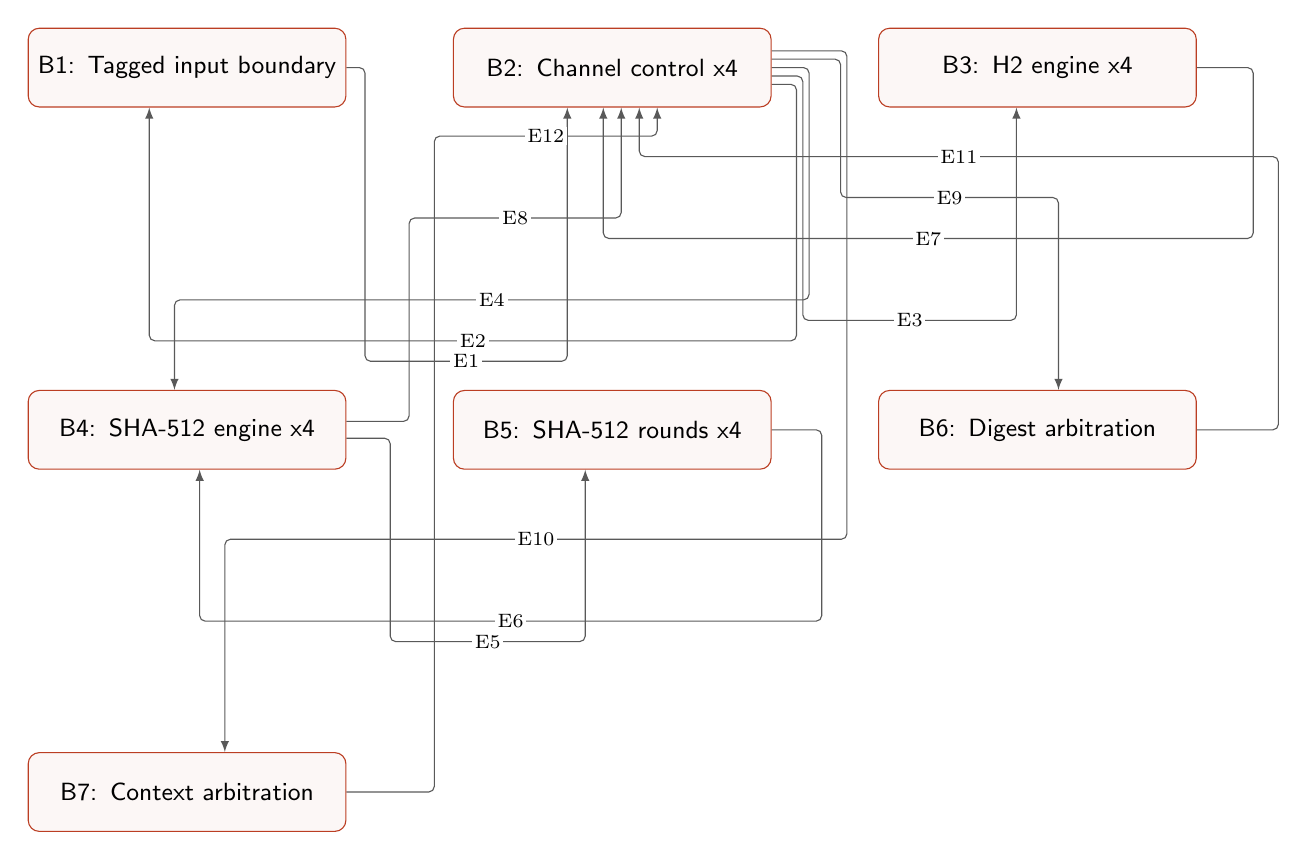
\begin{tikzpicture}[every node/.style={font=\small\sffamily},>=latex]

\node[draw=vulcan,rounded corners,fill=vulcan!4,text width=3.8cm,minimum height=1cm,align=center] (b0) at (0.0,0.0) {B1: Tagged input boundary};

\node[draw=vulcan,rounded corners,fill=vulcan!4,text width=3.8cm,minimum height=1cm,align=center] (b1) at (5.4,0.0) {B2: Channel control x4};

\node[draw=vulcan,rounded corners,fill=vulcan!4,text width=3.8cm,minimum height=1cm,align=center] (b2) at (10.8,0.0) {B3: H2 engine x4};

\node[draw=vulcan,rounded corners,fill=vulcan!4,text width=3.8cm,minimum height=1cm,align=center] (b3) at (0.0,-4.6) {B4: SHA-512 engine x4};

\node[draw=vulcan,rounded corners,fill=vulcan!4,text width=3.8cm,minimum height=1cm,align=center] (b4) at (5.4,-4.6) {B5: SHA-512 rounds x4};

\node[draw=vulcan,rounded corners,fill=vulcan!4,text width=3.8cm,minimum height=1cm,align=center] (b5) at (10.8,-4.6) {B6: Digest arbitration};

\node[draw=vulcan,rounded corners,fill=vulcan!4,text width=3.8cm,minimum height=1cm,align=center] (b6) at (0.0,-9.2) {B7: Context arbitration};

\begin{pgfonlayer}{connections}

\draw[->,black!65,rounded corners=2pt] ([yshift=0.000cm]b0.east) -- (2.260,0.000) -- (2.260,-3.730) -- coordinate[midway] (e0) (4.829,-3.730) -- ([xshift=-0.571cm]b1.south);

\draw[->,black!65,rounded corners=2pt] ([yshift=-0.213cm]b1.east) -- (7.740,-0.213) -- (7.740,-3.470) -- coordinate[midway] (e1) (-0.480,-3.470) -- ([xshift=-0.480cm]b0.south);

\draw[->,black!65,rounded corners=2pt] ([yshift=-0.107cm]b1.east) -- (7.820,-0.107) -- (7.820,-3.210) -- coordinate[midway] (e2) (10.533,-3.210) -- ([xshift=-0.267cm]b2.south);

\draw[->,black!65,rounded corners=2pt] ([yshift=0.000cm]b1.east) -- (7.900,0.000) -- (7.900,-2.950) -- coordinate[midway] (e3) (-0.160,-2.950) -- ([xshift=-0.160cm]b3.north);

\draw[->,black!65,rounded corners=2pt] ([yshift=-0.107cm]b3.east) -- (2.580,-4.707) -- (2.580,-7.290) -- coordinate[midway] (e4) (5.057,-7.290) -- ([xshift=-0.343cm]b4.south);

\draw[->,black!65,rounded corners=2pt] ([yshift=0.000cm]b4.east) -- (8.060,-4.600) -- (8.060,-7.030) -- coordinate[midway] (e5) (0.160,-7.030) -- ([xshift=0.160cm]b3.south);

\draw[->,black!65,rounded corners=2pt] ([yshift=0.000cm]b2.east) -- (13.540,0.000) -- (13.540,-2.170) -- coordinate[midway] (e6) (5.286,-2.170) -- ([xshift=-0.114cm]b1.south);

\draw[->,black!65,rounded corners=2pt] ([yshift=0.107cm]b3.east) -- (2.820,-4.493) -- (2.820,-1.910) -- coordinate[midway] (e7) (5.514,-1.910) -- ([xshift=0.114cm]b1.south);

\draw[->,black!65,rounded corners=2pt] ([yshift=0.107cm]b1.east) -- (8.300,0.107) -- (8.300,-1.650) -- coordinate[midway] (e8) (11.067,-1.650) -- ([xshift=0.267cm]b5.north);

\draw[->,black!65,rounded corners=2pt] ([yshift=0.213cm]b1.east) -- (8.380,0.213) -- (8.380,-5.990) -- coordinate[midway] (e9) (0.480,-5.990) -- ([xshift=0.480cm]b6.north);

\draw[->,black!65,rounded corners=2pt] ([yshift=0.000cm]b5.east) -- (13.860,-4.600) -- (13.860,-1.130) -- coordinate[midway] (e10) (5.743,-1.130) -- ([xshift=0.343cm]b1.south);

\draw[->,black!65,rounded corners=2pt] ([yshift=0.000cm]b6.east) -- (3.140,-9.200) -- (3.140,-0.870) -- coordinate[midway] (e11) (5.971,-0.870) -- ([xshift=0.571cm]b1.south);

\end{pgfonlayer}

\begin{pgfonlayer}{edge labels}

\node[fill=white,inner sep=1pt,font=\scriptsize] at (e0) {E1};

\node[fill=white,inner sep=1pt,font=\scriptsize] at (e1) {E2};

\node[fill=white,inner sep=1pt,font=\scriptsize] at (e2) {E3};

\node[fill=white,inner sep=1pt,font=\scriptsize] at (e3) {E4};

\node[fill=white,inner sep=1pt,font=\scriptsize] at (e4) {E5};

\node[fill=white,inner sep=1pt,font=\scriptsize] at (e5) {E6};

\node[fill=white,inner sep=1pt,font=\scriptsize] at (e6) {E7};

\node[fill=white,inner sep=1pt,font=\scriptsize] at (e7) {E8};

\node[fill=white,inner sep=1pt,font=\scriptsize] at (e8) {E9};

\node[fill=white,inner sep=1pt,font=\scriptsize] at (e9) {E10};

\node[fill=white,inner sep=1pt,font=\scriptsize] at (e10) {E11};

\node[fill=white,inner sep=1pt,font=\scriptsize] at (e11) {E12};

\end{pgfonlayer}

\end{tikzpicture}\end{center}

{\small Functional block map, not a gate-level netlist. Edge identifiers match the directed relationships below. Crossings do not denote junctions; separate attachment points preserve arrow directions.}

{\small\begin{longtable}{@{}L{0.24\textwidth}L{0.7\textwidth}@{}}\toprule

\textbf{Block} & \textbf{Responsi\allowbreak{}bility}\\\midrule\endhead

B1: Tagged input boundary & Routes message,\allowbreak{} key and command handshak\allowbreak{}es to the addresse\allowbreak{}d channel; returns readines\allowbreak{}s from that channel only.\\[3pt]

B2: Channel control x4 & Owns algorith\allowbreak{}m selectio\allowbreak{}n,\allowbreak{} command priority,\allowbreak{} fault isolatio\allowbreak{}n,\allowbreak{} context-envelope validati\allowbreak{}on and inactive-engine cleanup.\\[3pt]

B3: H2 engine x4 & Preserve\allowbreak{}s SHA-256,\allowbreak{} long-key HMAC normaliz\allowbreak{}ation,\allowbreak{} cached inner/\allowbreak{}outer seeds and original context processi\allowbreak{}ng.\\[3pt]

B4: SHA-512 engine x4 & Owns beat staging,\allowbreak{} 128-byte block collecti\allowbreak{}on,\allowbreak{} 128-bit byte count,\allowbreak{} chaining state,\allowbreak{} padding and snapshot\allowbreak{}s.\\[3pt]

B5: SHA-512 rounds x4 & Performs 80 iterativ\allowbreak{}e 64-bit rounds with a sixteen-word sliding schedule and separate feed-forward completi\allowbreak{}on.\\[3pt]

B6: Digest arbitrat\allowbreak{}ion & Locks one pending tagged digest until retireme\allowbreak{}nt and advances an independ\allowbreak{}ent round-robin pointer.\\[3pt]

B7: Context arbitrat\allowbreak{}ion & Independ\allowbreak{}ently locks one tagged 2304-bit snapshot until retireme\allowbreak{}nt.\\[3pt]

\bottomrule\end{longtable}}

{\small\begin{longtable}{@{}L{0.24\textwidth}L{0.7\textwidth}@{}}\toprule

\textbf{Directed relation\allowbreak{}ship} & \textbf{Meaning}\\\midrule\endhead

E1: B1 to B2 & Selected message,\allowbreak{} key and command transfer\allowbreak{}s\\[3pt]

E2: B2 to B1 & Selected-channel readines\allowbreak{}s\\[3pt]

E3: B2 to B3 & SHA/\allowbreak{}HMAC traffic and control\\[3pt]

E4: B2 to B4 & SHA-512 traffic and control\\[3pt]

E5: B4 to B5 & Prepared block,\allowbreak{} chain and launch\\[3pt]

E6: B5 to B4 & Feed-forward state and register\allowbreak{}ed completi\allowbreak{}on\\[3pt]

E7: B3 to B2 & H2 digest,\allowbreak{} snapshot and status\\[3pt]

E8: B4 to B2 & SHA-512 digest,\allowbreak{} snapshot and status\\[3pt]

E9: B2 to B6 & Selected-algorith\allowbreak{}m pending digest\\[3pt]

E10: B2 to B7 & Envelope\allowbreak{}d pending snapshot\\[3pt]

E11: B6 to B2 & Digest retireme\allowbreak{}nt\\[3pt]

E12: B7 to B2 & Snapshot retireme\allowbreak{}nt\\[3pt]

\bottomrule\end{longtable}}

\section{Interfaces and configuration}

{\small\begin{longtable}{@{}L{0.2\textwidth}L{0.12\textwidth}L{0.1\textwidth}L{0.48\textwidth}@{}}\toprule

\textbf{Signal /\allowbreak{} group} & \textbf{Directio\allowbreak{}n} & \textbf{Width} & \textbf{Contract}\\\midrule\endhead

clk,\allowbreak{} rst\_\allowbreak{}n & Input & 1 bit each & Rising-edge clock and asynchro\allowbreak{}nous active-low reset. While reset is asserted,\allowbreak{} every public ready,\allowbreak{} valid,\allowbreak{} payload,\allowbreak{} tag,\allowbreak{} algorith\allowbreak{}m and error output is zero.\\[3pt]

s\_\allowbreak{}valid,\allowbreak{} s\_\allowbreak{}ready,\allowbreak{} s\_\allowbreak{}channel,\allowbreak{} s\_\allowbreak{}data,\allowbreak{} s\_\allowbreak{}keep,\allowbreak{} s\_\allowbreak{}last & Input except output s\_\allowbreak{}ready & 1,\allowbreak{} 1,\allowbreak{} 2,\allowbreak{} 32,\allowbreak{} 4,\allowbreak{} 1 bits & Message stream. Transfer occurs only on a rising edge with valid and ready asserted. Channel indices are 0–3. Leading bytes start at data[\allowbreak{}31:24]\allowbreak{}; keep masks 1000,\allowbreak{} 1100,\allowbreak{} 1110 and 1111 encode one through four bytes.\\[3pt]

k\_\allowbreak{}valid,\allowbreak{} k\_\allowbreak{}ready,\allowbreak{} k\_\allowbreak{}channel,\allowbreak{} k\_\allowbreak{}data,\allowbreak{} k\_\allowbreak{}keep,\allowbreak{} k\_\allowbreak{}last & Input except output k\_\allowbreak{}ready & 1,\allowbreak{} 1,\allowbreak{} 2,\allowbreak{} 32,\allowbreak{} 4,\allowbreak{} 1 bits & HMAC key stream using the same byte and mask conventi\allowbreak{}on. Enabled during KEY\_\allowbreak{}LOAD; key completi\allowbreak{}on produces no digest.\\[3pt]

cmd\_\allowbreak{}valid,\allowbreak{} cmd\_\allowbreak{}ready,\allowbreak{} cmd\_\allowbreak{}channel,\allowbreak{} cmd\_\allowbreak{}op,\allowbreak{} cmd\_\allowbreak{}context & Input except output cmd\_\allowbreak{}ready & 1,\allowbreak{} 1,\allowbreak{} 2,\allowbreak{} 3,\allowbreak{} 2304 bits & Commands: 0 SHA\_\allowbreak{}INIT,\allowbreak{} 1 KEY\_\allowbreak{}LOAD,\allowbreak{} 2 HMAC\_\allowbreak{}INIT,\allowbreak{} 3 SAVE,\allowbreak{} 4 RESTORE,\allowbreak{} 5 CANCEL,\allowbreak{} 6 SHA512\_\allowbreak{}INIT. Accepted opcode 7 faults the addresse\allowbreak{}d channel. An accepted command suppress\allowbreak{}es same-channel stream transfer\allowbreak{}s.\\[3pt]

m\_\allowbreak{}valid,\allowbreak{} m\_\allowbreak{}ready,\allowbreak{} m\_\allowbreak{}channel,\allowbreak{} m\_\allowbreak{}alg,\allowbreak{} m\_\allowbreak{}digest & Output except input m\_\allowbreak{}ready & 1,\allowbreak{} 1,\allowbreak{} 2,\allowbreak{} 2,\allowbreak{} 512 bits & Locked digest response. Algorith\allowbreak{}m codes are 0 SHA-256,\allowbreak{} 1 HMAC-SHA-256 and 2 SHA-512; 3 is reserved. SHA-256/\allowbreak{}HMAC occupy bits [\allowbreak{}255:0]\allowbreak{} with zero upper bits. Digest bytes follow publishe\allowbreak{}d big-endian order.\\[3pt]

ctx\_\allowbreak{}valid,\allowbreak{} ctx\_\allowbreak{}ready,\allowbreak{} ctx\_\allowbreak{}channel,\allowbreak{} ctx\_\allowbreak{}data & Output except input ctx\_\allowbreak{}ready & 1,\allowbreak{} 1,\allowbreak{} 2,\allowbreak{} 2304 bits & Independ\allowbreak{}ent locked context response. The channel tag is outside the serializ\allowbreak{}ed state,\allowbreak{} enabling migratio\allowbreak{}n.\\[3pt]

error & Output & 4 bits & One sticky fault bit per channel. A faulty operatio\allowbreak{}n emits no digest; only CANCEL or reset recovers the channel.\\[3pt]

\bottomrule\end{longtable}}

{\small\begin{longtable}{@{}L{0.23\textwidth}L{0.12\textwidth}L{0.57\textwidth}@{}}\toprule

\textbf{Paramete\allowbreak{}r} & \textbf{Default} & \textbf{Meaning /\allowbreak{} supporte\allowbreak{}d values}\\\midrule\endhead

PARTIAL\_\allowbreak{}BEATS & 0 & Legal integer values are exactly 0 and 1,\allowbreak{} both exercise\allowbreak{}d on H3 and standalo\allowbreak{}ne H2. Value 0 requires full nonfinal beats and permits a zero-byte final beat only for an empty message/\allowbreak{}key. Value 1 permits leading partial nonfinal beats and zero-byte final terminat\allowbreak{}ors. Sparse masks remain invalid. Values -1 and 2 were explicit\allowbreak{}ly rejected with PARAMETE\allowbreak{}R ERROR and nonzero simulati\allowbreak{}on exit. Channel count is fixed at four.\\[3pt]

\bottomrule\end{longtable}}

\section{Behavior and corner cases}

\subsection{Collection and concurrency}

Each active channel has one beat stage and one block buffer. A beat captured at E0 first drains at E1; four bytes finish at E4,\allowbreak{} with no replacement on E4. A crossing beat pauses across block compression without losing bytes. Command,\allowbreak{} key and message ports may transfer simultaneously to different channels. A pending response blocks further work on its channel,\allowbreak{} but other channels can continue to their own response storage. No second message enters a channel before its prior digest retires.

\subsection{Exact cryptographic arithmetic}

SHA-256 and SHA-512 follow FIPS 180-4; HMAC-SHA-256 follows RFC 2104/\allowbreak{}RFC 4231,\allowbreak{} hashing keys longer than 64 bytes. SHA-512 uses eight 64-bit chaining words,\allowbreak{} standard IV/\allowbreak{}constants,\allowbreak{} 128-byte blocks and 80 rounds with modulo-2\textasciicircum{}64 addition. Its schedule is W[\allowbreak{}t]\allowbreak{}=\allowbreak{}sigma1(\allowbreak{}W[\allowbreak{}t-2]\allowbreak{})\allowbreak{}+\allowbreak{}W[\allowbreak{}t-7]\allowbreak{}+\allowbreak{}sigma0(\allowbreak{}W[\allowbreak{}t-15]\allowbreak{})\allowbreak{}+\allowbreak{}W[\allowbreak{}t-16]\allowbreak{},\allowbreak{} where sigma0 uses ROTR1/\allowbreak{}ROTR8/\allowbreak{}SHR7 and sigma1 uses ROTR19/\allowbreak{}ROTR61/\allowbreak{}SHR6. Large sigmas use rotations 28/\allowbreak{}34/\allowbreak{}39 and 14/\allowbreak{}18/\allowbreak{}41. Ch and Maj use the standard bitwise definitions.

\subsection{Padding and length limits}

SHA-512 appends 0x80,\allowbreak{} zeros and the complete 128-bit big-endian bit length. Residual lengths 112–127 require an extra padding block; an exactly full final data block precedes a fresh padding block. The full 128-bit byte counter rejects prospective counts above 2\textasciicircum{}125-1. SHA-256 permits at most 2\textasciicircum{}61-1 bytes; HMAC message length is limited to 2\textasciicircum{}61-65 bytes to account for its inner prefix.

\subsection{Algorithm and key lifetime}

Reset/\allowbreak{}CANCEL selects empty SHA-256 and clears keys. INIT/\allowbreak{}KEY\_\allowbreak{}LOAD at a nonempty quiescent prefix faults rather than discarding it. HMAC\_\allowbreak{}INIT requires a valid key. Same-domain commands preserve parent key-cache semantics. Entering SHA-512 clears inactive SHA/\allowbreak{}HMAC state and keys; returning to HMAC therefore requires a new or restored key. Digest retirement prepares another empty message in the same algorithm. CANCEL can interrupt collection,\allowbreak{} key loading or compression,\allowbreak{} but is backpressured while any channel response is pending.

\subsection{Response order and timing}

Independent digest/\allowbreak{}context round-robin pointers start at channel 0. An unlocked arbiter samples pending requests at an edge,\allowbreak{} locks the first cyclic candidate,\allowbreak{} and holds all fields until handshake. Retirement advances the pointer to winner+\allowbreak{}1; selection occurs on the following edge,\allowbreak{} producing one selection bubble. A continuously pending channel waits at most three other retirements,\allowbreak{} assuming eventual consumer readiness. Order is strict per channel,\allowbreak{} not globally by submission. Compression start at E0 yields SHA-256 done after E65 and SHA-512 done after E81; controllers consume registered completion later. End-to-end latency additionally includes collection and arbitration.

\subsection{Context serialization and validation}

SAVE/\allowbreak{}RESTORE require an unstaged,\allowbreak{} noncompressing,\allowbreak{} nonfinal,\allowbreak{} non-key-loading prefix without a pending response. SAVE freezes the channel until context retirement; RESTORE may atomically replace a nonempty prefix. The H3 envelope has payload [\allowbreak{}2047:0]\allowbreak{},\allowbreak{} magic [\allowbreak{}2079:2048]\allowbreak{}=\allowbreak{}0x52485633,\allowbreak{} version [\allowbreak{}2087:2080]\allowbreak{}=\allowbreak{}1,\allowbreak{} algorithm [\allowbreak{}2089:2088]\allowbreak{},\allowbreak{} and zero [\allowbreak{}2303:2090]\allowbreak{}. SHA/\allowbreak{}HMAC retain the exact H2 payload in [\allowbreak{}1535:0]\allowbreak{},\allowbreak{} with zero upper payload and matching mode. SHA-512 stores count [\allowbreak{}127:0]\allowbreak{},\allowbreak{} used [\allowbreak{}135:128]\allowbreak{},\allowbreak{} chain [\allowbreak{}647:136]\allowbreak{},\allowbreak{} buffer [\allowbreak{}1671:648]\allowbreak{},\allowbreak{} and zero upper payload. Used must equal count modulo block size,\allowbreak{} unused buffer bytes must be zero,\allowbreak{} and initial chains must match the required IV/\allowbreak{}seed. Invalid headers,\allowbreak{} reserved fields,\allowbreak{} lengths or consistency checks fault without partial installation. Zero-extended original H2 contexts are accepted.

\section{Verification methods and measured results}

\subsection{Exact digests and mandatory boundary coverage}

\textbf{Method.} Real Icarus 12.0 compilation/\allowbreak{}vvp execution with Python hashlib/\allowbreak{}hmac expectations,\allowbreak{} literal published SHA vectors,\allowbreak{} six RFC 4231 HMAC vectors per run,\allowbreak{} and an independent compression reference for synthetic high counts.

\textbf{Result.} Seeds 17,\allowbreak{} 89 and 2026 each passed under both parameter settings: 581 comparisons per strict-mode run and 587 per partial-mode run,\allowbreak{} totaling 3,\allowbreak{}504 with zero mismatches. Every run completed 312 directed,\allowbreak{} 72 random and three 65,\allowbreak{}536-byte messages,\allowbreak{} plus additional cases. All channels exercised SHA-512 boundaries including 111/\allowbreak{}112/\allowbreak{}127/\allowbreak{}128/\allowbreak{}129 bytes; random lengths covered 0–8192 bytes. These totals exclude benchmarks and compatibility checks.

{\small Evidence: E014,\allowbreak{} E015,\allowbreak{} E016,\allowbreak{} E017,\allowbreak{} E024}

\subsection{Protocol isolation,\allowbreak{} state migration and recovery}

\textbf{Method.} Public-handshake scoreboarding with mandatory event bins for masks,\allowbreak{} commands,\allowbreak{} stalls,\allowbreak{} arbitration,\allowbreak{} reset/\allowbreak{}cancel and restored high-count states.

\textbf{Result.} All six runs passed required bins,\allowbreak{} including four pending digests,\allowbreak{} late-arrival locked grants,\allowbreak{} digest/\allowbreak{}context stalls of at least 64 cycles,\allowbreak{} simultaneous retirements,\allowbreak{} and source bubbles. Each run included 15 context migrations,\allowbreak{} 15 uninterrupted continuations and seven high-count comparisons. Prefixes were 0,\allowbreak{}1,\allowbreak{}63,\allowbreak{}64,\allowbreak{}65 for SHA/\allowbreak{}HMAC and 0,\allowbreak{}1,\allowbreak{}127,\allowbreak{}128,\allowbreak{}129 for SHA-512. Malformed contexts,\allowbreak{} all keep masks/\allowbreak{}finalities,\allowbreak{} length overflow and isolated faults were exercised without missing,\allowbreak{} extra or duplicate responses.

{\small Evidence: E024}

\subsection{Parent compatibility}

\textbf{Method.} Byte comparison against supplied reference RTL and independent standalone H2 simulations under both legal parameters,\allowbreak{} including bidirectional H2/\allowbreak{}H3 context interchange.

\textbf{Result.} All six copied modules were byte-identical. Compatibility completed 244 digest comparisons: 118 strict-mode standalone comparisons,\allowbreak{} 122 partial-mode standalone comparisons and four H2-to-H3 import comparisons. H3-to-H2 restores were included in the standalone counts. Key reuse/\allowbreak{}replacement,\allowbreak{} original contexts,\allowbreak{} mask errors and cancellation passed.

{\small Evidence: E003,\allowbreak{} E004,\allowbreak{} E005,\allowbreak{} E006,\allowbreak{} E007,\allowbreak{} E008,\allowbreak{} E025}

\subsection{Defect-sensitive checking}

\textbf{Method.} Four isolated mutations in disposable RTL copies,\allowbreak{} each compiled and executed against targeted functional workloads.

\textbf{Result.} All four mutants were rejected functionally: SHA-512 arithmetic corruption and padding threshold 112-to-113 by DIGEST\_\allowbreak{}ORACLE; channel association corruption by EXTRA\_\allowbreak{}DIGEST/\allowbreak{}DIGEST\_\allowbreak{}ORACLE; stalled-output corruption by DIGEST\_\allowbreak{}STABILITY. Compile failures were not counted as detection.

{\small Evidence: E026}

\subsection{Measured latency and aggregate throughput}

\textbf{Method.} Twenty-four deterministic single-algorithm workloads plus one mixed workload,\allowbreak{} with ready outputs and pre-NBA rising-edge handshake timestamps. Each length/\allowbreak{}algorithm used 16 messages on one channel or 16 per channel on four channels.

\textbf{Result.} For lengths 0/\allowbreak{}112/\allowbreak{}128/\allowbreak{}1024 bytes,\allowbreak{} elapsed cycles for one/\allowbreak{}four active channels were SHA-256: 1169/\allowbreak{}1265,\allowbreak{} 4481/\allowbreak{}5825,\allowbreak{} 5905/\allowbreak{}7441,\allowbreak{} 39281/\allowbreak{}50897; HMAC: 2241/\allowbreak{}2337,\allowbreak{} 5553/\allowbreak{}6897,\allowbreak{} 6977/\allowbreak{}8513,\allowbreak{} 40353/\allowbreak{}51969; SHA-512: 1425/\allowbreak{}1521,\allowbreak{} 4961/\allowbreak{}6353,\allowbreak{} 5313/\allowbreak{}6897,\allowbreak{} 32753/\allowbreak{}44753. At 1024 bytes,\allowbreak{} cycles/\allowbreak{}message were respectively 2455.0625/\allowbreak{}795.265625,\allowbreak{} 2522.0625/\allowbreak{}812.015625 and 2047.0625/\allowbreak{}699.265625; cycles/\allowbreak{}byte were 2.39752/\allowbreak{}0.77663,\allowbreak{} 2.46295/\allowbreak{}0.79298 and 1.99908/\allowbreak{}0.68288. Aggregate throughput ratios were approximately 3.09,\allowbreak{} 3.11 and 2.93,\allowbreak{} not fourfold. The mixed batch used channels SHA-256/\allowbreak{}HMAC/\allowbreak{}SHA-512/\allowbreak{}SHA-256,\allowbreak{} 16 messages each at 128 bytes: 8192 bytes in 8449 cycles,\allowbreak{} 132.015625 cycles/\allowbreak{}message and 0.96958 bytes/\allowbreak{}cycle.

{\small Evidence: E024}

\subsection{Latency convention and excluded setup costs}

\textbf{Method.} Intervals span post-setup MARK 1 to final-retirement MARK 2; reset and key setup are excluded. Per-message timestamps and all 25 metric records are retained in evidence/\allowbreak{}behavior/\allowbreak{}attempt-2487c27399324546b98b90dd6d6e4a77/\allowbreak{}measurements.json.

\textbf{Result.} Single-channel first-beat-to-valid latencies at lengths 0/\allowbreak{}112/\allowbreak{}128/\allowbreak{}1024 were SHA-256 72/\allowbreak{}279/\allowbreak{}368/\allowbreak{}2454 cycles,\allowbreak{} HMAC 139/\allowbreak{}346/\allowbreak{}435/\allowbreak{}2521,\allowbreak{} and SHA-512 88/\allowbreak{}309/\allowbreak{}331/\allowbreak{}2046. Last-beat-to-valid latencies were 72/\allowbreak{}75/\allowbreak{}144/\allowbreak{}144,\allowbreak{} 139/\allowbreak{}142/\allowbreak{}211/\allowbreak{}211 and 88/\allowbreak{}174/\allowbreak{}176/\allowbreak{}176. With ready consumers,\allowbreak{} retirement shares the sampled valid edge. Reset occupied three cycles; total pre-steady setup was 4/\allowbreak{}16 cycles for SHA workloads and 244/\allowbreak{}976 for HMAC. The deterministic HMAC key-setup interval was 242 cycles per channel. Empty-message cycles/\allowbreak{}byte is undefined,\allowbreak{} not zero.

{\small Evidence: E024}

\subsection{Synthesizability and retained structure}

\textbf{Method.} Yosys 0.33 hierarchy checks,\allowbreak{} process/\allowbreak{}memory lowering,\allowbreak{} optimization,\allowbreak{} generic synthesis,\allowbreak{} consistency assertions and retained preflatten connectivity inspection under both legal parameters.

\textbf{Result.} Both configurations passed latch,\allowbreak{} hierarchy,\allowbreak{} driver and loop checks with substantive state and output-driving logic. RTL totals were 66,\allowbreak{}341 bytes,\allowbreak{} 1,\allowbreak{}632 lines and 11 modules. Each elaboration contained 41 instances including top,\allowbreak{} with four connected channel/\allowbreak{}H2/\allowbreak{}SHA-512 engine hierarchies. Generic leaf cells were 422,\allowbreak{}518 for parameter 0 and 422,\allowbreak{}458 for parameter 1; both had 55,\allowbreak{}126 state cells and zero remaining memories after lowering. Standalone H2 elaborated successfully.

{\small Evidence: E027}

\subsection{Source-only portable reproduction}

\textbf{Method.} Copied only declared RTL,\allowbreak{} design documents,\allowbreak{} Python verification sources and reference RTL into a fresh project-relative directory,\allowbreak{} then invoked the shipped entry point.

\textbf{Result.} The clean-copy run passed 61 digest comparisons covering all algorithms,\allowbreak{} context migration and output stalls,\allowbreak{} plus illegal-parameter rejection and default H3 synthesis. This is a measured portable subset,\allowbreak{} not another full six-run regression. Python 3.12.3,\allowbreak{} Icarus 12.0 and Yosys 0.33 were recorded prerequisites.

{\small Evidence: E028}

\section{Integration and use}

Use rtl/\allowbreak{}*\allowbreak{}.sv with top rivet\_\allowbreak{}h3\_\allowbreak{}top; select rivet\_\allowbreak{}h2\_\allowbreak{}top for the unchanged standalone interface. design/\allowbreak{}SPEC.md defines ports,\allowbreak{} context layouts and cycle rules; design/\allowbreak{}ARCHITECTURE.md describes hierarchy and storage. Static elaboration command: \texttt{iverilog -g2012 -t null -s rivet\_\allowbreak{}h3\_\allowbreak{}top -s rivet\_\allowbreak{}h2\_\allowbreak{}top rtl/\allowbreak{}*\allowbreak{}.sv}.


Assert reset before traffic. Reset starts empty SHA-256; use SHA512\_\allowbreak{}INIT for SHA-512,\allowbreak{} or KEY\_\allowbreak{}LOAD followed by the complete key stream and HMAC\_\allowbreak{}INIT for HMAC. Hold valid,\allowbreak{} channel and payload stable until transfer. Maintain software ordering independently per channel and consume tags rather than assuming global submission order.


From the project root,\allowbreak{} run \texttt{python3 tests/\allowbreak{}verify.py --check behavior --out evidence/\allowbreak{}behavior},\allowbreak{} \texttt{python3 tests/\allowbreak{}verify.py --check compatibility --out evidence/\allowbreak{}compatibility},\allowbreak{} \texttt{python3 tests/\allowbreak{}verify.py --check defects --out evidence/\allowbreak{}defects},\allowbreak{} \texttt{python3 tests/\allowbreak{}verify.py --check synthesis --out evidence/\allowbreak{}synthesis},\allowbreak{} and \texttt{python3 tests/\allowbreak{}verify.py --check portable --out evidence/\allowbreak{}portable}. No arguments runs the complete suite into a fresh directory. Existing outputs are retained; receipts identify any fresh retry directory.


Required external executables are python3,\allowbreak{} iverilog,\allowbreak{} vvp and yosys. Generated receipts retain source hashes,\allowbreak{} exact commands,\allowbreak{} configuration,\allowbreak{} timestamps,\allowbreak{} exit/\allowbreak{}timeout information and raw-log locations. Source inputs do not depend on generated executables,\allowbreak{} existing evidence,\allowbreak{} runtime metadata or the final report.


\section{Limitations and acceptance boundary}

This is RTL-IP delivery with simulation-cycle and generic-synthesis evidence. No technology-mapped area,\allowbreak{} clock frequency,\allowbreak{} timing closure,\allowbreak{} power,\allowbreak{} FPGA operation or silicon measurement is established.


Replication does not remove shared-input bandwidth limits and can increase individual message latency under interleaved traffic. Throughput results apply to the recorded deterministic workloads and ready consumers; they are not universal speedup guarantees.


HMAC-SHA-512,\allowbreak{} configurable channel count,\allowbreak{} multiple queued messages per channel and global submission-order retirement are unsupported. Arbitration fairness requires eventual consumer readiness for a finite cycle bound.


Contexts are unauthenticated functional state and may contain HMAC-derived seeds. Syntactic validation does not establish confidentiality,\allowbreak{} integrity,\allowbreak{} side-channel resistance or security certification.


Verification is extensive simulation and synthesis checking,\allowbreak{} not exhaustive formal proof. Extreme length behavior was checked using validated synthetic contexts and independent compression expectations,\allowbreak{} not physically streamed maximum-length messages.


\appendix\section{Source inventory}

Production inventory: 11 Verilog/\allowbreak{}SystemVerilog files; 1586 nonblank,\allowbreak{} non-comment lines. Source size is not a correctness or quality metric.

{\small\begin{longtable}{@{}L{0.61\textwidth}L{0.15\textwidth}L{0.15\textwidth}@{}}\toprule

\textbf{Producti\allowbreak{}on file} & \textbf{Physical lines} & \textbf{Code lines}\\\midrule\endhead

rtl/\allowbreak{}rivet\_\allowbreak{}h2\_\allowbreak{}compress.sv & 169 & 164\\[3pt]

rtl/\allowbreak{}rivet\_\allowbreak{}h2\_\allowbreak{}context.sv & 61 & 59\\[3pt]

rtl/\allowbreak{}rivet\_\allowbreak{}h2\_\allowbreak{}hmac.sv & 66 & 64\\[3pt]

rtl/\allowbreak{}rivet\_\allowbreak{}h2\_\allowbreak{}schedule.sv & 39 & 37\\[3pt]

rtl/\allowbreak{}rivet\_\allowbreak{}h2\_\allowbreak{}stream.sv & 81 & 79\\[3pt]

rtl/\allowbreak{}rivet\_\allowbreak{}h2\_\allowbreak{}top.sv & 380 & 368\\[3pt]

rtl/\allowbreak{}rivet\_\allowbreak{}h3\_\allowbreak{}channel.sv & 173 & 167\\[3pt]

rtl/\allowbreak{}rivet\_\allowbreak{}h3\_\allowbreak{}sha512.sv & 299 & 293\\[3pt]

rtl/\allowbreak{}rivet\_\allowbreak{}h3\_\allowbreak{}sha512\_\allowbreak{}compress.sv & 184 & 180\\[3pt]

rtl/\allowbreak{}rivet\_\allowbreak{}h3\_\allowbreak{}sha512\_\allowbreak{}schedule.sv & 38 & 37\\[3pt]

rtl/\allowbreak{}rivet\_\allowbreak{}h3\_\allowbreak{}top.sv & 142 & 138\\[3pt]

\bottomrule\end{longtable}}

\section{Verification record index}

{\small\begin{longtable}{@{}L{0.57\textwidth}L{0.16\textwidth}L{0.17\textwidth}@{}}\toprule

\textbf{Recorded check} & \textbf{Outcome} & \textbf{Executio\allowbreak{}n time (\allowbreak{}s)\allowbreak{}}\\\midrule\endhead

behavior & passed & 660.751\\[3pt]

compatib\allowbreak{}ility & passed & 11.256\\[3pt]

defect\_\allowbreak{}sensitiv\allowbreak{}ity & passed & 1.528\\[3pt]

synthesi\allowbreak{}s & passed & 268.078\\[3pt]

portable\_\allowbreak{}reproduc\allowbreak{}tion & passed & 132.643\\[3pt]

\bottomrule\end{longtable}}

Execution times include tool and provider waiting; they are not hardware latency or model utilization.

{\small\begin{longtable}{@{}L{0.12\textwidth}L{0.82\textwidth}@{}}\toprule

\textbf{Referenc\allowbreak{}e} & \textbf{Original project-relative record}\\\midrule\endhead

E003 & rtl/\allowbreak{}rivet\_\allowbreak{}h2\_\allowbreak{}compress.sv\\[3pt]

E004 & rtl/\allowbreak{}rivet\_\allowbreak{}h2\_\allowbreak{}context.sv\\[3pt]

E005 & rtl/\allowbreak{}rivet\_\allowbreak{}h2\_\allowbreak{}hmac.sv\\[3pt]

E006 & rtl/\allowbreak{}rivet\_\allowbreak{}h2\_\allowbreak{}schedule.sv\\[3pt]

E007 & rtl/\allowbreak{}rivet\_\allowbreak{}h2\_\allowbreak{}stream.sv\\[3pt]

E008 & rtl/\allowbreak{}rivet\_\allowbreak{}h2\_\allowbreak{}top.sv\\[3pt]

E014 & tests/\allowbreak{}bridge.py\\[3pt]

E015 & tests/\allowbreak{}referenc\allowbreak{}e.py\\[3pt]

E016 & tests/\allowbreak{}scenario\allowbreak{}s.py\\[3pt]

E017 & tests/\allowbreak{}verify.py\\[3pt]

E024 & .vulcan/\allowbreak{}engineer\allowbreak{}ing/\allowbreak{}run-0001/\allowbreak{}attempt-0005/\allowbreak{}stdout.log\\[3pt]

E025 & .vulcan/\allowbreak{}engineer\allowbreak{}ing/\allowbreak{}run-0001/\allowbreak{}attempt-0006/\allowbreak{}stdout.log\\[3pt]

E026 & .vulcan/\allowbreak{}engineer\allowbreak{}ing/\allowbreak{}run-0001/\allowbreak{}attempt-0007/\allowbreak{}stdout.log\\[3pt]

E027 & .vulcan/\allowbreak{}engineer\allowbreak{}ing/\allowbreak{}run-0001/\allowbreak{}attempt-0008/\allowbreak{}stdout.log\\[3pt]

E028 & .vulcan/\allowbreak{}engineer\allowbreak{}ing/\allowbreak{}run-0001/\allowbreak{}attempt-0009/\allowbreak{}stdout.log\\[3pt]

\bottomrule\end{longtable}}

\section{Document provenance}

Engineering was independently accepted for the recorded source and evidence identity. This is not exhaustive proof, hardware deployment or physical signoff. The companion REPORT.md records the exact report approval and source manifest, and links the English/Chinese journeys containing original failures and interventions. A report number identifies a generation attempt, not a new hardware revision.

No developer attribution was supplied; none has been inferred.

\end{document}
